\documentclass[12]{article}
\usepackage[margin=1in]{geometry}
\usepackage{graphicx, float,amsmath, physics, amssymb}
\usepackage{physics,hyperref,subcaption}
\hypersetup{
    colorlinks=true,
    linkcolor=black,
    filecolor=black,      
    urlcolor=blue,
    citecolor=black,
}

\begin{document}
\begin{flushright}
Tim Skaras

Advisor: Professor Mustafa Amin
\end{flushright}

\begin{center}
{\LARGE Faraday Wave Experiment}
\end{center}

\section{Introduction}

Bose-Einstein Condensation (BEC) is a state of matter in boson gases that results when atoms, cooled very close to absolute zero, abruptly accumulate in their ground state \cite{schroeder1999introduction}. This state of matter has been experimentally realized using various atomic vapors \cite{pethick2008bose}. In particular, a laboratory here at Rice led by Professor Randall Hulet has studied Bose-Einstein Condensation in lithium. Professor Hulet's lab is able to tune the interaction strength between atoms by exploiting a shallow zero-crossing of a Feshbach resonance, and, due to nonlinearity, this can result in rich dynamics such as the creation of matter-wave soliton trains \cite{nguyen2017formation}. Because it is difficult to study nonlinear systems analytically, computational tools have been important for understanding the behavior of these systems.

\subsection{Project Overview}

More recently, Professor Hulet's lab has performed experiments on the emergence of Faraday Waves in a Bose-Einstein Condensate by periodically modulating the scattering length for these atoms. In these experiments, they have modulated the scattering length periodically for a fixed period of time. Then after holding the scattering length constant, they observe that perturbations of particular wavenumbers will grow rapidly, resulting in the emergence of faraday waves.

Using a mean field theory, it can be shown that the dynamics of a Bose-Einstein condensate are governed by the time-dependent Gross-Pitaevskii Equation \cite{pethick2008bose}
\begin{equation}
i \hbar \frac{\partial \psi(\mathbf{r}, t)}{\partial t}=-\frac{\hbar^{2}}{2 m} \nabla^{2} \psi(\mathbf{r}, t)+V(\mathbf{r}) \psi(\mathbf{r}, t)+ g|\psi(\mathbf{r}, t)|^{2} \psi(\mathbf{r}, t), \quad \quad g \equiv 4 \pi \hbar^{2} a_{s} / m
\label{DimGPE3D}
\end{equation}
\nolinebreak
where $\psi$ is a field describing the number density of atoms in real space, hence the total particle number $N$ satisfies
\begin{equation}
\int_{\mathbb{R}^{3}} d \mathbf{r}|\psi(\mathbf{r})|^{2} = N
\end{equation}
The parameter $g$ corresponds to the interaction strength between atoms ($g>0$ corresponding to repulsive interactions and $g < 0$ corresponding to attractive interactions), and is defined in terms of the scattering length $a_s$ and the atomic mass $m$.

In this project, I numerically solve this nonlinear, partial differential equation assuming a cigar-shaped trapping potential in three spatial dimensions to computationally confirm recent experimental results from Professor Hulet's lab by showing that the BEC's perturbations in Fourier space grow in the expected way.

\section{Methods}

\subsection{Dimensionless GPE}

Though the form given for the Gross-Pitaevskii equation in (\ref{DimGPE3D}) is physically correct, the units in which the equation has been expressed are not appropriate for the time and length scale of our problem. To remedy this, we will first scale the field
\begin{equation}
\frac{\psi}{\sqrt{N}} \rightarrow \psi
\end{equation}
which now gives the PDE
\begin{equation}
i \hbar \frac{\partial \psi(\mathbf{r}, t)}{\partial t}=-\frac{\hbar^{2}}{2 m} \nabla^{2} \psi(\mathbf{r}, t)+V(\mathbf{r}) \psi(\mathbf{r}, t)+ gN|\psi(\mathbf{r}, t)|^{2} \psi(\mathbf{r}, t), \quad \quad g \equiv 4 \pi \hbar^{2} a_{s} / m
\label{GPEUnity}
\end{equation}
with a normalization condition that is set to unity
\begin{equation}
\int_{\mathbb{R}^{3}} d \mathbf{r}|\psi(\mathbf{r})|^{2} = 1
\end{equation}
To make the GPE dimensionless, we stipulate that the potential is harmonic
\begin{equation}
V(\textbf{r}) = \frac{m}{2}\left(\omega_{x}^{2} x^{2}+\omega_{y}^{2} y^{2}+\omega_{z}^{2} z^{2}\right)
\end{equation}
and then choose a convenient characteristic length $a_0$ and scale our coordinates as follows
\begin{equation}
\omega_{x} t \rightarrow t, \quad \mathbf{r} / a_{0} \rightarrow \mathbf{r}, \quad a_{0}^{3 / 2} \psi \rightarrow \psi \quad \text { where } \quad a_{0} \equiv \sqrt{\frac{\hbar }{ m \omega_{x}}}
\label{scaling}
\end{equation}
Plugging (\ref{scaling}) into (\ref{GPEUnity}) and simplifying we find the GPE in dimensionless form can be written as
\begin{equation}
i \frac{\partial \psi(\mathbf{r}, t)}{\partial t}= -\frac{1}{2 } \nabla^{2} \psi(\mathbf{r}, t)+V(\mathbf{r}) \psi(\mathbf{r}, t)+ gN|\psi(\mathbf{r}, t)|^{2} \psi(\mathbf{r}, t), \quad \quad g \equiv 4 \pi a_{s}
\label{GPE3D}
\end{equation}
where the potential has been scaled so that one of the trapping frequencies is unity
\begin{equation*}
V(\textbf{r}) = \frac{1}{2}\left( x^{2}+\gamma_{y}^{2} y^{2}+\gamma_{z}^{2} z^{2}\right), \quad \gamma_y \equiv \frac{\omega_y}{\omega_x}, \quad \gamma_z \equiv \frac{\omega_z}{\omega_x}
\end{equation*}
For the Faraday Wave experiment that we will be considering, the trapping potential is cylindrically symmetric with $j\omega_x = \omega_y$, so the trapping potential is really
\begin{equation}
V(\textbf{r}) = \frac{1}{2}\left( \rho^{2}+\gamma_{z}^{2} z^{2}\right), \quad \rho^2 = x^2 + y^2
\end{equation}

\subsection{Numerical Methods}
To solve this nonlinear PDE, I use a time-splitting spectral (TSSP) method while assuming periodic boundary conditions. The general idea behind applying this method is that some operators on the RHS of (\ref{GPE3D}) are easy to apply in momentum space (e.g., the second order derivative) and some are easy to apply in position space (e.g., the potential term). To exploit this fact, this method involves shifting the wave function solution between its real space and momentum space representation via fourier transformation and applying each operator component in the space it is most easily applied. 

Before I can start solving the nonlinear PDE, however, I must find the correct initial condition. These experiments in Hulet's lab are performed on BEC that is very close to its ground state. The ground state for the GPE is not known analytically in this trapping potential, so I will use finite difference methods to implement the imaginary-time propagation method \cite{chiofalo2000ground, muruganandam2009fortran}, which will allow me to numerically calculate the ground state.

The TSSP method is described in detail in \cite{bao2003numerical} for a one dimensional version of the GPE, and the method can be straightforwardly generalized to three spatial dimensions without affecting the method's validity. The advantages of this method are multifold: the TSSP method is unconditionally stable, time reversible, time-transverse invariant, conserves particle number, and is second order accurate in space and time \cite{bao2003numerical}. One noteworthy drawback is that this method is not symplectic, i.e., it does not conserve energy.

Time reversible means that if the solution $\psi_{n+1}$ at $t_{n+1}$ is obtained by applying the TSSP method to the solution $\psi_n$ at $t_n$, then the past state can be re-obtained from $\psi_{n+1}$ by using TSSP with time step $-\Delta t = -(t_{n+1} - t_n)$. Time-transverse invariance or gauge invariance refers to the property of the GPE that if $V \rightarrow V + \alpha$ where $\alpha \in \mathbb{R}$, then the solution $\psi \rightarrow \psi e^{i\alpha t}$, which implies that number density of atoms $|\psi|^2$ is unchanged under this transformation. This method respects this property by producing the corresponding changes in $\psi$ when $V$ is transformed in this way \cite{antoine2013computational}.

\subsection{Implementation and Validation}

I have implemented this spectral method in Python\footnote{My \href{https://github.com/TimSkaras/GPE-SpectralMethod}{github} repository}. I used the CuPy package\footnote{\href{https://cupy.chainer.org}{CuPy website}} to implement this method because this package provides a NumPy-like environment that performs computations on a GPU. This allowed my code to acheive considerable speedup (almost an order of magnitude for certain problems) over a serial implementation. I will now consider some of the test cases that I have used to ensure I have correctly implemented the time-splitting spectral method and the imaginary-time propagation method.

\subsubsection{Homogeneous Solution}

It can be trivially verified that
\begin{equation}
\psi(t) = A e^{-i g|A|^2 t}, \quad A \in \mathbb{C}
\end{equation}
is a solution to (\ref{GPE3D}). It should be noted that the method will accurately solve a constant intial condition ($\psi(\textbf{x},0) = A$) only when the time step is small compared to the period of oscillation which is determined by angular frequency $\omega = g |A|^2$. In the file \href{https://github.com/TimSkaras/GPE-SpectralMethod/blob/master/Tests/homogeneous_test.py}{homogeneous\_test.py}, I solve a homogeneous initial condition with $A = \frac{1}{2}$ and $g = 10$ thus giving $T = \frac{2\pi}{\omega} = 2.51$. Our time step is $\Delta t \approx 0.0179$. For more details on parameters, see the file linked in this document.

After solving the problem with these initial conditions until $t = 2.5$. When the code is run using a GPU, the maximum error at any one gridpoint is on the order of $10^{-14}$ and the normalization loss ratio (the change in the normalization divided by the norm at $t=0$) is also on the order of $10^{-14}$. Running the code in serial gives a max error and norm loss ratio of the same order of magnitude.

\subsubsection{Plane Wave}

It is also possible to show that the Gross-Pitaevskii Equation admits a plane wave solution with the form
\begin{equation}
\psi(\textbf{r},t) = Ae^{i(\textbf{k} \dotproduct \textbf{r} - \omega t)}, \quad A \in \mathbb{C}
\end{equation}
provided that $\omega$ and $\vec{k}$ satisfy the dispersion relation
\begin{equation}
\omega(\textbf{k}) = \frac{1}{2}|\textbf{k}|^2 + g \abs{A}^2
\end{equation}
In the file \href{https://github.com/TimSkaras/GPE-SpectralMethod/blob/master/Tests/homogeneous_test.py}{planewave\_test.py}, I use this analytic solution to again test the accuracy of my solver. I use the same value for $A$ and $g$ but with $\vec{k} = (\frac{2\pi}{L_x}, 2\frac{2\pi}{L_y},3\frac{2\pi}{L_z})$ the period is now $T = \frac{2\pi}{\omega} = 1.97$. Solving this plane wave initial condition until $t = 2.5$ gives a max error on the order of $10^{-13}$ and a norm loss ratio on the order of $10^{-14}$. Changing from GPU to serial has no significant effect on the error and loss of normalization.

Because this initial condition is spatially varying, it gives us a little more information on how well the solver is working. The spatial derivative in (\ref{GPE3D}) is handled entirely separately from the potential and nonlinear terms. The TSSP method splits (\ref{GPE3D}) into two equations that each be solved exactly and then combines the splitting steps together using Strang splitting to give a second-order accurate solution. The equation with the Laplacian is solved using fourier transforms, and in the code this is handled with FFT. This test and the previous one are useful for testing these different components and isolating which part of the solver has a problem if any.
 
\subsubsection{Thomas-Fermi Ground State}

The previous two test cases are meant to ensure that the code is correctly solving equation (\ref{GPE3D}), but it is also necessary to test that I have correctly implemented the imaginary-time propagation method. Though we have no exact ground state to which we can compare our numerical result, it is possible to write down an approximate ground state for certain limiting cases of the GPE \cite{bao2003numerical, bao2003ground}.

As explained in the references just cited, a stationary solution $\phi(\textbf{x})$ of the GPE can be written as
\begin{equation}
\psi(\textbf{r},t)  = e^{-i\mu t}\phi(\textbf{r})
\label{stationary}
\end{equation}
where $\mu$ is the chemical potential. Plugging (\ref{stationary}) into (\ref{GPE3D}) gives us the equation $\phi(\textbf{x})$ must satisfy to be a stationary solution
\begin{equation}
\mu \phi(\mathbf{r})=-\frac{1}{2} \nabla^{2} \phi(\mathbf{r})+V(\mathbf{r}) \phi(\mathbf{r})+ g|\phi(\mathbf{r})|^{2} \phi(\mathbf{r})
\label{StationaryGPE}
\end{equation}
with the normalization condition
\begin{equation}
\int_{\mathbb{R}^{3}}|\phi(\mathbf{r})|^{2} d \mathbf{r}=1.
\label{NormCondition}
\end{equation}
The ground state is the stationary solution satsifying (\ref{StationaryGPE}) and (\ref{NormCondition}) while also minimizing the energy functional
\begin{equation}
E[\phi] := \int_{\mathbb{R}^{3}} \left[ \frac1{2} |\nabla \phi|^{2}  + V(\textbf{r})|\phi|^{2} + \frac{g}{2}|\phi|^{4} \right] d \mathbf{r}
\label{Energy}
\end{equation}
This ground state solution is unique if we also require that $\phi$ be real. In the strongly-interacting regime where $g N \gg a_{0}$ and $g > 0$, the ground state can be approximated as 
\begin{equation}
\mu_{g}=\frac{1}{2}\left(\frac{15 gN \gamma_y\gamma_{z}}{4 \pi}\right)^{2 / 5}, \phi_{g}(\mathbf{x})=\left\{\begin{array}{ll}{\sqrt{\frac{\mu_{g}-V(\mathbf{x}) }{gN}},} & {V(\mathbf{x})<\mu_{g}} \\ {0,} & {\text { otherwise }}\end{array}\right.
\label{StrongGS}
\end{equation}
This approximate ground state is known as the Thomas-Fermi ground state. It can be derived from the Thomas-Fermi approximtion where the kinetic term in (\ref{GPE3D}) is dropped from the equation.

In the file \href{https://github.com/TimSkaras/GPE-SpectralMethod/blob/master/Tests/TFgs_test.py}{TFgs\_test.py}, I have used my implementation of the imaginary-time propagation method to find the ground state in a trap with $\omega_x = \omega_y = \omega_z = 1$ and $gN = 2000$. On a grid of points $64 \times 64 \times 64$ points, I have compared my numerically calculated ground state with the analytic approximation given in (\ref{StrongGS}), and I have provided a plot of each in figure \ref{fig:TFgs}. 

\begin{figure}[H]
    \begin{subfigure}[t]{0.5\textwidth}
        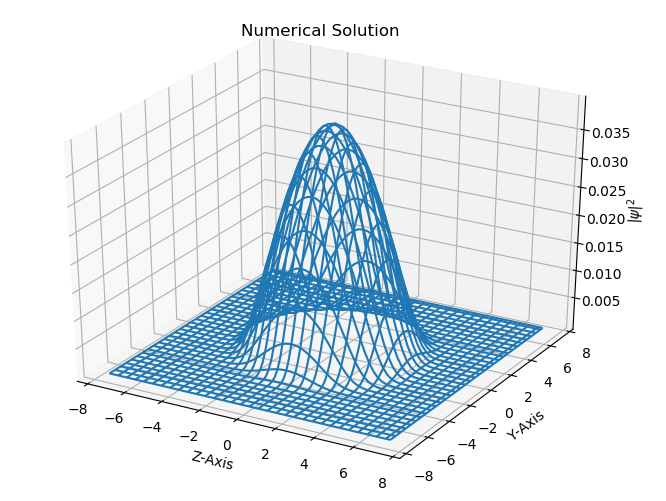
\includegraphics[scale=0.35]{Plots/TFgsNumerical}
        \caption{}
    \end{subfigure}\hfill
    \begin{subfigure}[t]{0.45\textwidth}
        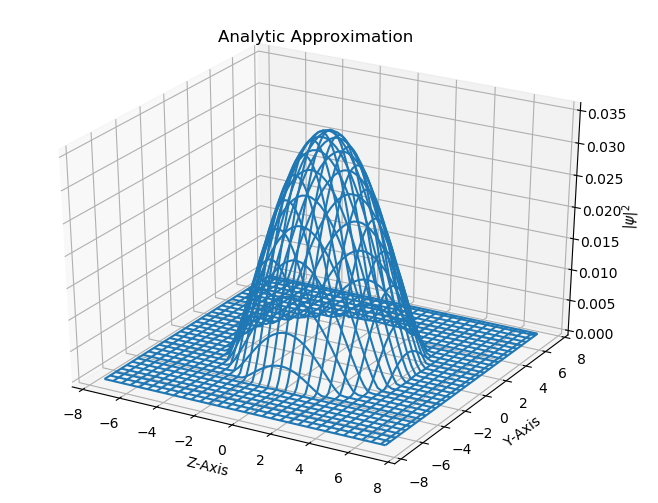
\includegraphics[scale=0.35]{Plots/TFgsAnalytic}
        \caption{}
    \end{subfigure}
    \caption{These are plots of $|\psi|^2$ for the numerically calculated solution (a) and the analytic approximation (b). The x-dimension has been integrated out to make plotting possible. The two are very similar execpt at the boundary where the analytic aproximation becomes zero.}
    \label{fig:TFgs}
\end{figure}

To compare how close the numerical solution is the analytic approximation, I used equation (\ref{Energy}) to calculate the ground state energy for each. The numerical solution has an energy of 8.28 and the analytic approximation has an energy of 8.37, and the max error between the wavefunction for each was 0.010. 

These figures are not as promising as the tests for the GPE solver were, but there may be good reason for this. Bao et al. \cite{bao2003ground} write that the energy of the Thomas-Fermi ground state is actually infinite, namely
\begin{equation}
E[\phi_g] = +\infty
\end{equation}
due to the low regularity of $\phi_g$ at the free boundary where $V(x) = \mu_g$. To remedy this issue, an interface layer has to be constructed at this boundary to improve the accuracy of the approximation.

\section{Results}

\subsection{Experiment Description}

\subsection{Analytic Prediction}

\subsection{Computational Results}

\bibliographystyle{abbrv}
\bibliography{FaradayExperimentBib}

\end{document}